%Abstract like thing?
%The binding corrections to the gyromagnetic ratio $g$ are investigated for a particle of arbitrary spin.  The corrections are worked %out for specific spin-half and spin-one theories, before considering the more general case.  By considering the constraints lying upon %the relativistic theory, an effective nonrelativistic Lagrangian is developed.

\chapter{Introduction}


A way to calculate the binding corrections to the spin $g$-factor of a charged particle of arbitrary spin is desired.



The $g$ factor in this sense can be defined by the energy separation of two particles which differ only by spin orientation.  (For particles in a bound state, a $g$-factor can be defined with respect to the angular momentum of the particle as well.)  A free electron, with its spin oriented along the same axis as a weak magnetic field $B_z\hat{z}$, has energy
\beq
 E = - \gv{\mu} \cdot \v{B} = - g \frac{e}{2m}s_z B_z
\eeq
The difference between such an electron and one with its spin flipped is then
\beq
	\delta E = - g \frac{e}{m}s_z B_z = -g \mu_B B
\eeq


The general definition of the $g$-factor then follows -- the energy difference between two particles with spin projection parallel and anti-parallel to a small constant magnetic field will be proportional to $ - \mu_B B$, and the coefficient of this difference defines the $g$-factor.


\section{The free $g$-factor}
The most well known $g$-factor is that of the free electron.  It may be calculated from the Lagrangian of QED.
\beq
	\mathcal{L} = \Psibar \left( i \partial \cdot \gamma - e A \cdot \gamma - m \right ) \Psi
\eeq
The Dirac equation itself predicts a magnitude of $g=2$.  

When calculated in the framework of QED, there will be corrections to this ``natural'' value of $2$.  The $g$-factor being determined by the behavior of the electron in a infinitesimal magnetic field, the relevant QED calculation is the process

\mbox{
\begin{minipage}{1in}
  \begin{center} 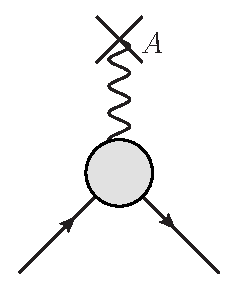
\includegraphics[scale=0.5]{eps/QED-static-field-blob} \end{center} 
\end{minipage}
=
\begin{minipage}{1in}
   \begin{center}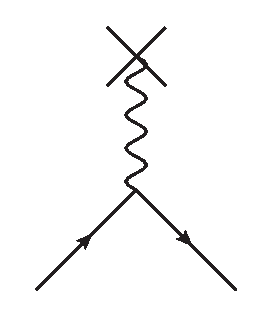
\includegraphics[scale=0.5]{eps/QEDfund}\end{center} 
\end{minipage}
+
\begin{minipage}{1in}
   \begin{center} 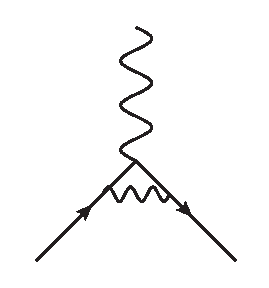
\includegraphics[scale=0.5]{eps/QEDloop1} \end{center} 
\end{minipage}
+
\begin{minipage}{1in}
   \begin{center} 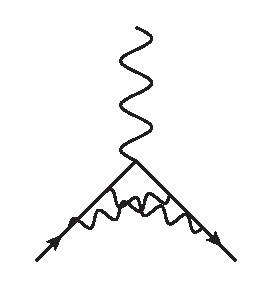
\includegraphics[scale=0.5]{eps/QEDloop2} \end{center} 
\end{minipage}
+ \hspace{2em} $\cdots$
 }
 
When only the fundamental vertex is calculated, the value of $2$ is obtained.  The additional loop diagrams such as illustrated above will introduce corrections to this quantity.  For an electron, these corrections will be quite small compared to the natural value of $2$.  
 
 
 
 This correction to the $g$-factor is related to the anomalous magnetic moment $a_e = (g-2)/2$.  Its calculation will be a series in the coupling constant $\alpha$.   (At very high orders additional interactions will enter into the calculation, but because of the light mass of the electron compared to other particles they are highly suppressed.)  The well known first order result is
 \beq
 	a_e = \frac{\alpha}{2\pi} + \mathcal{O}( \frac{\alpha^2}{4\pi^2})
 \eeq
The full value has been calculated to extremely high accuracy, such that the uncertainty in $g$ is 
\beq
	\frac{\Delta g}{g} \sim 10^{-13}
\eeq

It has also been measured with a similar accuracy.  A couple of the most recent measurements for the electron are
%FIXME find results
\beq
	g = 2.0-------    \hspace{2em} \delta = -- \text{(Hanneke, Fogwell, Gavielese)}
\eeq

Because both the experimental and theoretical values are known quite precisely, these measurements of the free electron's $g$-factor provide the best determination of the constant $\alpha$.  

For the electron, the leading order term came from the fundamental vertex, and the anomalous contribution coming from radiative corrections are relatively small.  In the more general case this is not true.  The proton has a $g$-factor of $\sim 5.6$, where because of its composite nature the anomalous part is quite large.

It is still necessarily the case that $g$ is determined by the same process as the electron.  And this process can be parametrized by two form factors, whose value wraps up the detailed information of the high energy physics or the small scale structure of the particle. 

\subsection{Bound $g$-factors}

Even when the free $g$ factor of a particle is known, there are corrections when the particle is placed into a bound state.  Consider again the simplee case of the electron, but this time it sits in a hydrogenic bound state.  It is immediately clear that the situation is much more complicated than the free case.  There are several additional scales to the problem, and so the expression for $g_b$ is no longer a series only in $\alpha$.
\begin{itemize}
  \item 	There are recoil corrections that occur when separating the internal degrees of freedom from the external motion of the whole bound system.  The related parameter is the mass ratio $m/M$	%TODO better to phrase in terms of reduced mass?
  \item 	The relativistic motion of the particle contributes binding corrections.  Because the velocity of a hydrogenic bound system is $v \sim Z\alpha$, corrections of this nature will be an expansion over $(Z\alpha)^2$.
  \item		There can be effects due to the finite size of the nucleus, although these are not considered in this work.
\end{itemize}
All of these are in addition to the radiative corrections discussed earlier; the full series will contain mixtures of all types of corrections at higher orders.

%XXX REF for Breit
The binding corrections for the electron with $g=2$ were first calculated by Breit (1928).  This can be done simply by taking the matrix element of the fundamental vertex (that responsible for the value $g=2$)  between the bound state wave functions.  This calculation of $\avg{ e\gamma \cdot A}$ gives
\beq 
	g_b = 2 \left( 1 - \frac{(Z\alpha)^2}{3} - \frac{(Z\alpha)^4}{12} \right )
\eeq



\subsection{Experimental relevance}
There are experiments involving hydrogenic $\hC$ and $\hO$ that require a precise theoretical determination of the bound $g$-factor.


A hydrogenic system is placed in a weak magnetic field $B$.  The spin flip frequency $\omega_L$ is measured, corresponding to transitions between Zeeman levels.  It is through this quantity that dependence on $g_b$ enters:
\beq
	\omega_L = g_b \frac{e}{2m_e} B
\eeq

The cyclotron frequency $\omega_C$ is
\beq
	\omega_C = (Z-1) \frac{eB}{M}
\eeq

So the ratio of these frequencies gives
\beq
	\frac{\omega_L}{\omega_C} = \frac{f_L}{f_C} = 
	g_b \frac{e}{2q} \frac{M}{m_e}
\eeq
This no longer depends on $B$, but does depend upon $g_b$ and the ratio of the electron mass ratio $m_e/M$.  If $g_b$ is known with sufficient precision, measuring this ratio is the best determination of $m_e/M$.

The best current measurements are, for $\hC$ ($Z=6$)
\beq
	 \frac{f_L}{f_C} = ~~~~~
\eeq

And for $\hO$ ($Z=8$)
\beq
		 \frac{f_L}{f_C} = ~~~~~
\eeq

With this generation of experiments the uncertainty is $\delta \sim 10^{-10}$, but in the future is expected to increase to $\delta \sim 10^{-12}$.  To fully exploit such sensitivity requires $g_b$ to be known with sufficient precision.

Here there is an issue connected with the overall spin magnitude of the nuclei.  In both $\hO$ and $\hC$, the nucleon spins are arranged such that the overall spin is $0$.  It is entirely plausible that the binding corrections to the $g$-factor could depend on the spin of the particles.  So some approach to this problem that works for nuclei of arbitrary spin would be useful.

%FIXME REF for E+G
There are already two extant approaches to this problem.  An method based on the Bargmann-Michel-Telegdi (BMT) equation was utilised by Eides and Grotch \cite{Eides:1997sq}.  Leading relativistic and recoil corrections are calculated, with the result that they are in fact independent of spin.  This follows from the form of the BMT equation, which itself carries no dependence on spin.  The leading order correction of to $g$ for a hydrogenic atom was found to be
\beq
	\Delta g_{EG} = (1 + Z)(Z\alpha)^2 \left( \frac{m_e}{M} \right )^2
\eeq 

In \cite{doi:10.1139/p02-112} Faustov and Martynenko used a quasipotential framework to calculate $g_b$.  Here the result was found to depend upon the spin of the particle.  For a spin-half particle there is agreement between this and the above approach, but clearly in general there is disagreement.   For a hydrogenic atom with a spin-0 nucleus, the result was
\beq
	\Delta g_{FM} = \frac{Z}{3} (Z\alpha)^2 \left( \frac{m_e}{M} \right )^2
\eeq
To give a concrete idea of the discrepancy produced by the methods, here are the numerical results pertinent to the previously mentioned experiments:  
\begin{center}
\begin{tabular}{r c c}
 					&	$\hC$						&	 $\hO$	\\	\hline
 $\Delta g_{EG}$		&	$ 0.28 \times 10^{-10}$ 	&	$ 0.36 \times 10^{-10}$	\\
 $\Delta g_{GM}$		&	$ 0.80 \times 10^{-11}$		&	$ 0.11 \times 10^{-10}$	\\
 Discrepancy			&	$ 0.2 \times 10^{-10}$		&	$ 0.25\times 10^{-10}$	\\
\end{tabular}
\end{center}

Such discrepancies are relevant to the sorts of experiments previously discussed, so a resolution to the situation is important.

\section{Attack}

%FIXME REF khriplovich reference, sp?
To resolve this disagreement, the following approach will be taken.  The starting point will be a relativistic description of the electromagnetic current for particles of arbitrary spin.  Just as for spin-half particles, all the details of the particles structure may be captured by form factors.  This follows the path laid out by Khriplovich (XXXX)

Fully relativistic theories being cumbersome to apply to bound state problems, an effective field theory approach is adopted.  A nonrelativistic Lagrangian for particles of arbitrary spin is constructed.  Then by considering the same physical process in the relativistic and nonrelativistic theory, the particular parameters of the NRQED Lagrangian will be determined.

With the NRQED Lagrangian determined to the order necessary, it may then be used to attack the bound state nature of the problem.  In a manner analogous to the calculation of the Breit potential (REF) an interaction Hamiltonian for the system can be developed.  Finally, this may be used to calculate $g_b$ at the necessary order.





